% !TEX program = xelatex
\documentclass[10pt,aspectratio=169]{beamer}
\usetheme{VK}
\usepackage{dsfont}
\usepackage{bm}
\usepackage{xunicode}
\usepackage{xltxtra}
\usepackage{xecyr}
\usepackage{listings}
\usepackage{tikz}
\usetikzlibrary{angles,quotes}
\usepackage{mwe}
\usepackage{multirow}
\usepackage{csquotes}
\usepackage[style=verbose-ibid,backend=bibtex]{biblatex}
\bibliography{references}


\date[]{}
\title[]{Программная реализация \linebreak
системы встроенного самотестирования \linebreak
для ARINC 653 ОСРВ}
\author[]{Иван Дорошенко, 4 курс}

% Закомментируйте эти строчки для того, 
% чтобы не указывать консультанта или руководителя
\newcommand{\supervisor}{Хорошилов А. В.}
\newcommand{\consultant}{Чепцов В. Ю.}
\date[]{16 апреля 2024 г.}

\begin{document}
\maketitle

% Все слайды определяются через \begin{frame}{Название слайда}
\begin{frame}{Архитектура ИМА}
    \textbf{Операционная система реального времени} (ОСРВ)~--- операционная система, способная обеспечить требуемый уровень сервиса в определённый промежуток времени.
    \textbf{Бортовые ОСРВ} используются для управления бортовым оборудованием.
    \skipline

    Одним из стандартов на программное обеспечение, используемое в бортовом оборудовании, является \textbf{ARINC 653}, регламентирующий разделение ресурсов между \textbf{разделами}, которые сопоставляются функциональным узлам.
\end{frame}

\begin{frame}{Планирование в ARINC 653}
    \begin{figure}[H]
        \centering
        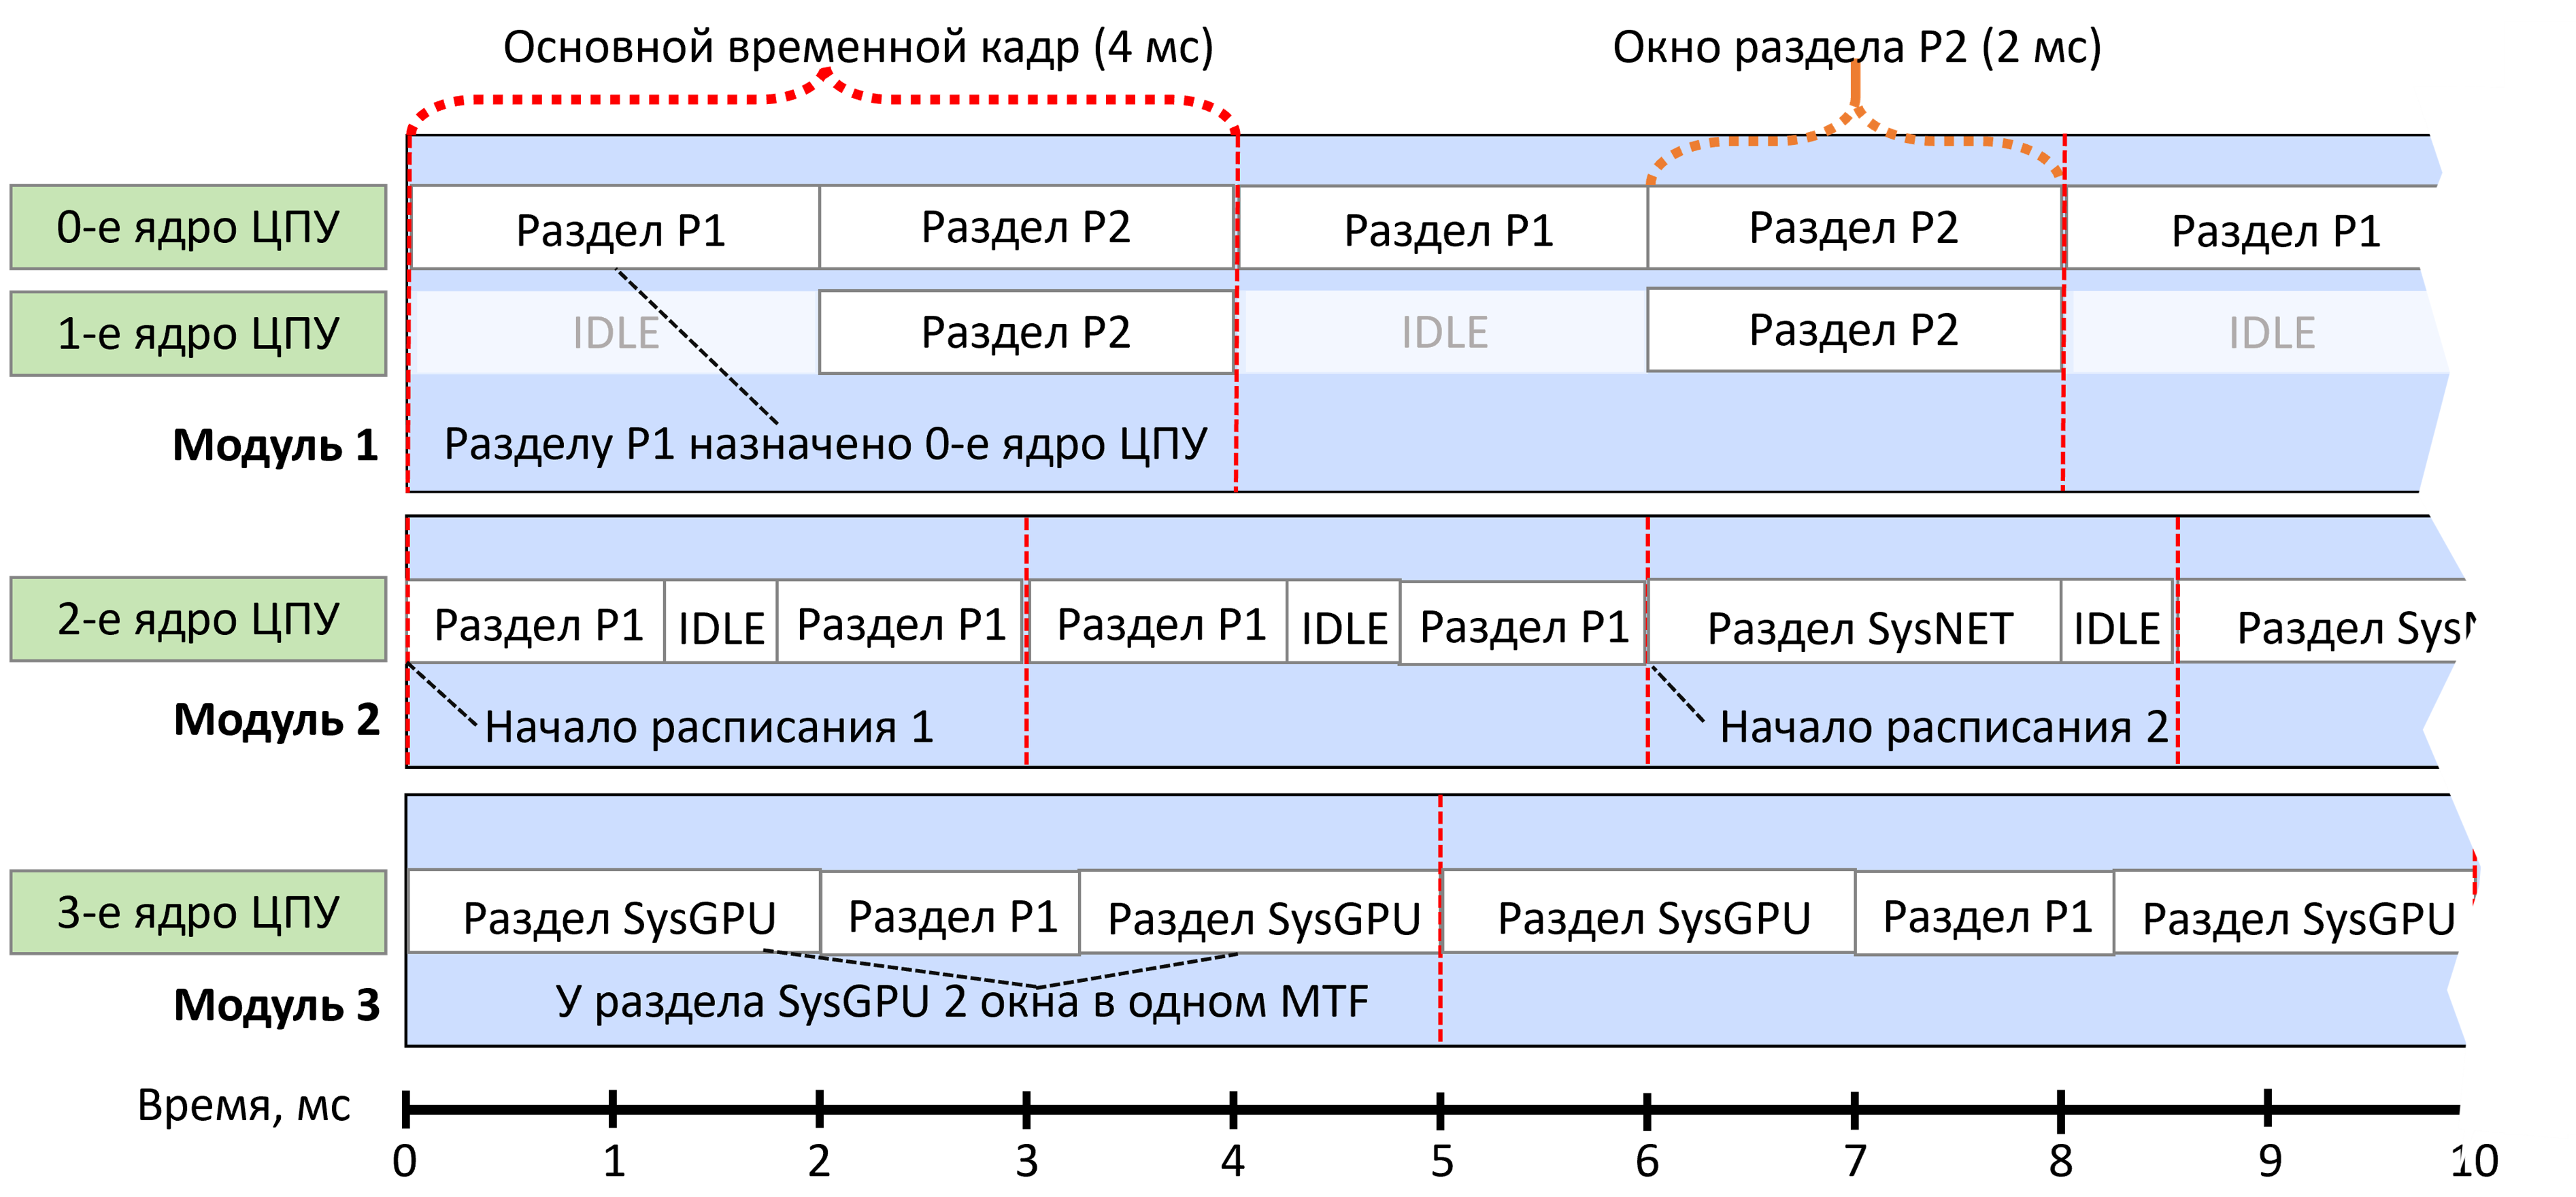
\includegraphics[width=10cm]{images/scheduling.png}
    \end{figure}
    \begin{itemize}
        \item Расписания распределяют время по окнам между разделами в рамках модуля.
        \item Окна расписания повторяются каждый основной временной кадр.
        \item Ядра ЦПУ назначаются разделу в рамках расписания.
    \end{itemize}
\end{frame}


\begin{frame}{Другие подобные слайды}
    Здесь могут содержаться другие слайды, которые определяются точно так же.
\end{frame}

% Эта команда вставляет последний слайд в докладе
\usebeamertemplate{endpage}

% Если нужно вынести слайд как дополнительный, чтобы можно было отвечать 
% с помощью него на вопросы, укажите в квадратных скобках [noframenumbering],
% а также добавить инструкцию \thispagestyle{empty}
\begin{frame}[noframenumbering]{Дополнительный слайд}
    \thispagestyle{empty}
    
    Здесь располагается дополнительная информация, которую не нужно рассказывать во время основного доклада, но которая может оказаться полезной для ответов на вопросы.
\end{frame}

\begin{frame}[noframenumbering]{Интересные факты}
    \thispagestyle{empty}
    
    \begin{enumerate}
        \item Чтобы в VS Code включить перенос длинных строк, нажмите Alt+Z (или Option+Z на macOS)
        \item Я использую расширение \LaTeX-Workshop в VS Code. Рекомендуется поставить в JSON-настройках значение \newline
        \texttt{"latex-workshop.latex.recipe.default": "latexmk (xelatex)",}
        \item Sample text
        \item Автор не несёт ответственности за взрыв мозга при попытке использовать этот шаблон, потому что сам разбирается в \LaTeX\ очень и очень плохо…
    \end{enumerate}
\end{frame}

\end{document}